\documentclass[12pt]{article}  % [12pt] option for the benefit of aging markers
\usepackage{amssymb,amsthm}    % amssymb package contains more mathematical symbols
\usepackage{graphicx}          % graphicx package enables you to paste in graphics
\usepackage[capposition=top]{floatrow}
\usepackage{setspace}
\usepackage{float}
\usepackage[backend=bibtex,sorting=nyt,firstinits=true]{biblatex}
\usepackage{hyperref}
\usepackage{longtable}
\usepackage{wrapfig}

\usepackage{lipsum}
\usepackage[margin=2cm]{geometry}

\addbibresource{references.bib}
\newcommand{\rid}[1]{\centering #1-\ifnum\value{requirement}<10 0\fi\arabic{requirement} \stepcounter{requirement}}


%%%%%%%%%%%%%%%%%%%%%%%%%%%%%%%%%%%%%%%%%
%										%
%     			Title					%
%										%
%%%%%%%%%%%%%%%%%%%%%%%%%%%%%%%%%%%%%%%%%
\title{Digital Lab Marking System \\~\\  \large{Heriot-Watt University} \\~\\ Final Year Dissertation}
\author{Lewis McNeill\\
supervised by
Peter J King}



\begin{document}
\maketitle
\pagenumbering{gobble}
\newpage

\doublespacing
\textbf{\Large{Declaration}} \\[2em]
I, Lewis Francis McNeill, confirm that this work submitted for assessment is my own and is expressed in my own words. Any references, made within it, of the works of other authors in any way (e.g., ideas, equations, figures, text, tables, programs) are properly acknowledged at any point of their use. A list of the references employed is included.
\\
\\
Signed: Lewis McNeill
\\
Date: \today



\newpage                 
\begin{abstract}

\noindent
The aim of this dissertation project is to replace the current system for the marking of computer labs with a new digital system. This will enable lecturers to create a marking scheme online. Lab helpers will select the student they are marking and the marking scheme will then be loaded, marks will be entered and then made immediately available for both student and lecturers to view. It will also provide useful statistics for both student and lecturers.

\end{abstract}

\newpage                  
\tableofcontents


%%%%%%%%%%%%%%%%%%%%%%%%%%%%%%%%%%%%%%%%%
%										%
%     		Introduction				%
%										%
%%%%%%%%%%%%%%%%%%%%%%%%%%%%%%%%%%%%%%%%%
\newpage     
\section{Aims, Objectives and Project Description}
\setcounter{page}{1}
\pagenumbering{arabic}

\subsection{Aim}
The aim of this dissertation is to design and implement a system for the digital marking and analysis of computer labs and to help improve the speed at which they are marked. The system will also provide useful statistics for both lecturers and students.

\subsection{Objectives}
\begin{itemize}
\item Simplify the way that labs marks are currently processed.
\item Allow lecturers to create marking schemes online that lab helps can access
\item Lab helpers can mark students in labs using marking schemes.
\item Develop a system that allows lab helpers to mark labs using an online application.
\item Allow students to see the mark they got from the lab instantly.
\item Provide useful statistics and graphs for lecturers.
\end{itemize}






%%%%%%%%%%%%%%%%%%%%%%%%%%%%%%%%%%%%%%%%%
%										%
%     	   Literature Review			%
%										%
%%%%%%%%%%%%%%%%%%%%%%%%%%%%%%%%%%%%%%%%%


\newpage
\section{Literature Review}
This section contains the current academic literature relating to anything relevant to current marking systems and the development of the new digital marking system.


\subsection{Marking Systems}

\subsubsection{Lecturer Based}
The way lecturer based marking works is that students complete their assignment, the lecturer or tutor marks it and provides result in a timely manner to help the student improve.\\
The advantage of this style of marking is that it provides useful feedback for individual students.
A downside to this style of marking is that the number of students increases on courses the amount of time required to mark assignments naturally takes longer and in some cases can actually cause marking to be scrapped completely \cite{brown_assessment_1999}. 


\subsubsection{Peer Based}
To cope with increasing class sizes some courses are beginning to move towards peer marking.\\
Peer marking system works by having students assess each other and some cases have the student think up their own marking criteria \cite{orsmond_use_2000}. This style allows for students to gain experience in evaluating other people's work, which some graduates feel is a necessary skill to have \cite{langan_insights_????}. Peer marking also deals with increasing amounts of students very well, this is because as the number students increase the number of marks also increases.  \\
Peer marking has its own set of problems for example, "Students may have a less well developed sense of the criteria compared to the lecturer which could lead to a lack of reliability of student marking." \cite{orsmond_use_2000}. \\


\newpage
\subsection{Digital Marking Systems}

\subsubsection{Reasons for Digital Marking}
Digital marking systems are designed to mirror current paper based marking systems but take advantage of the electronic environment \cite{heinrich_online_2003}. These systems help to reduce the increasing work caused by more and more students taking courses. Along with this it also allows administrative tasks associated with coursework to be automated enabling more time for other tasks.\cite{joy_effective_1998} 

\subsubsection{TurnItIn}
There currently exists an electronic plagiarism system called TurnItIn \cite{_turnitin_????} currently being used by many universities around the world. It allows students to upload their essay assignments online. it then checks for plagiarism in the document by searching the internet and using a large database of documents. After it process the document it assigns a plagiarism percentage and highlights any areas that were plagiarized. Lecturers can then login and view all the submitted documents and mark them online.\\
An article titled \citetitle{dahl_turnitin_2007} \cite{dahl_turnitin_2007} conducting a questionnaire found that students felt that the system was easy to use and more convenient than having to had to provide paper copies. It also found that 50\% agreed and 33.3\% of students prefered to have their grade shown online rather than have a cover sheet.



\newpage
\subsection{User Access Views}

Controlling the view that users have based on their access level is common practise, social media websites for instance allow users to limit what other users can see. This means that if another user is a friend then they can see there whole feed, while other users may only see their profile picture.

The patent titled \citetitle{baker_system_1997} \cite{baker_system_1997}, describes a system of limiting user web page access through the use of relation databases. The system would work by using two databases, one would hold a list of all the url's and associated access level, while second database would hold all the user id's along with and assigned access level. When a user requests a website the access level for the webpage and the user are looked up, if the user does not have the appropriate access they are denied permission to load the page.


\subsection{Custom Input Forms}

\subsubsection{SurveyMonkey}
Survey monkey \cite{finley_surveymonkey_1999} is an example of custom web forms being created by users. Founded by Ryan Finley in 1999 Survey Monkey enables users to create their own surveys and easily distribute them. It builds the surveys by letting the user select the contents of the question and what the response type will be: The user can also decide if the response are completely anonymous by default the participants ip address is stored when they complete the survey. The user can continue to add as many questions as they would like, even after the survey is initially created. After designing the survey the user chooses how they would like to have their survey distributed. The available options that can select are a web link, social media, email or embeddable on a website . 

When participants complete the survey their results are immediately stored and the results of the survey are visible to the user by login into their account on surveymonkey. They can choose to look at the responses individually or look at metrics about how participants responded.


\subsubsection{Customizing Forms In Electronic Mail Systems}
\noindent
The patent \citetitle{holt_customizing_2006} \cite{holt_customizing_2006} describes a process for user-customisable forms in an e-mail system where the administrator selects custom field types and behaviors.  For example current e-mail

\begin{wrapfigure}[7]{r}{0.5\textwidth}
\vspace*{-\baselineskip}
\begin{figure}[H]
  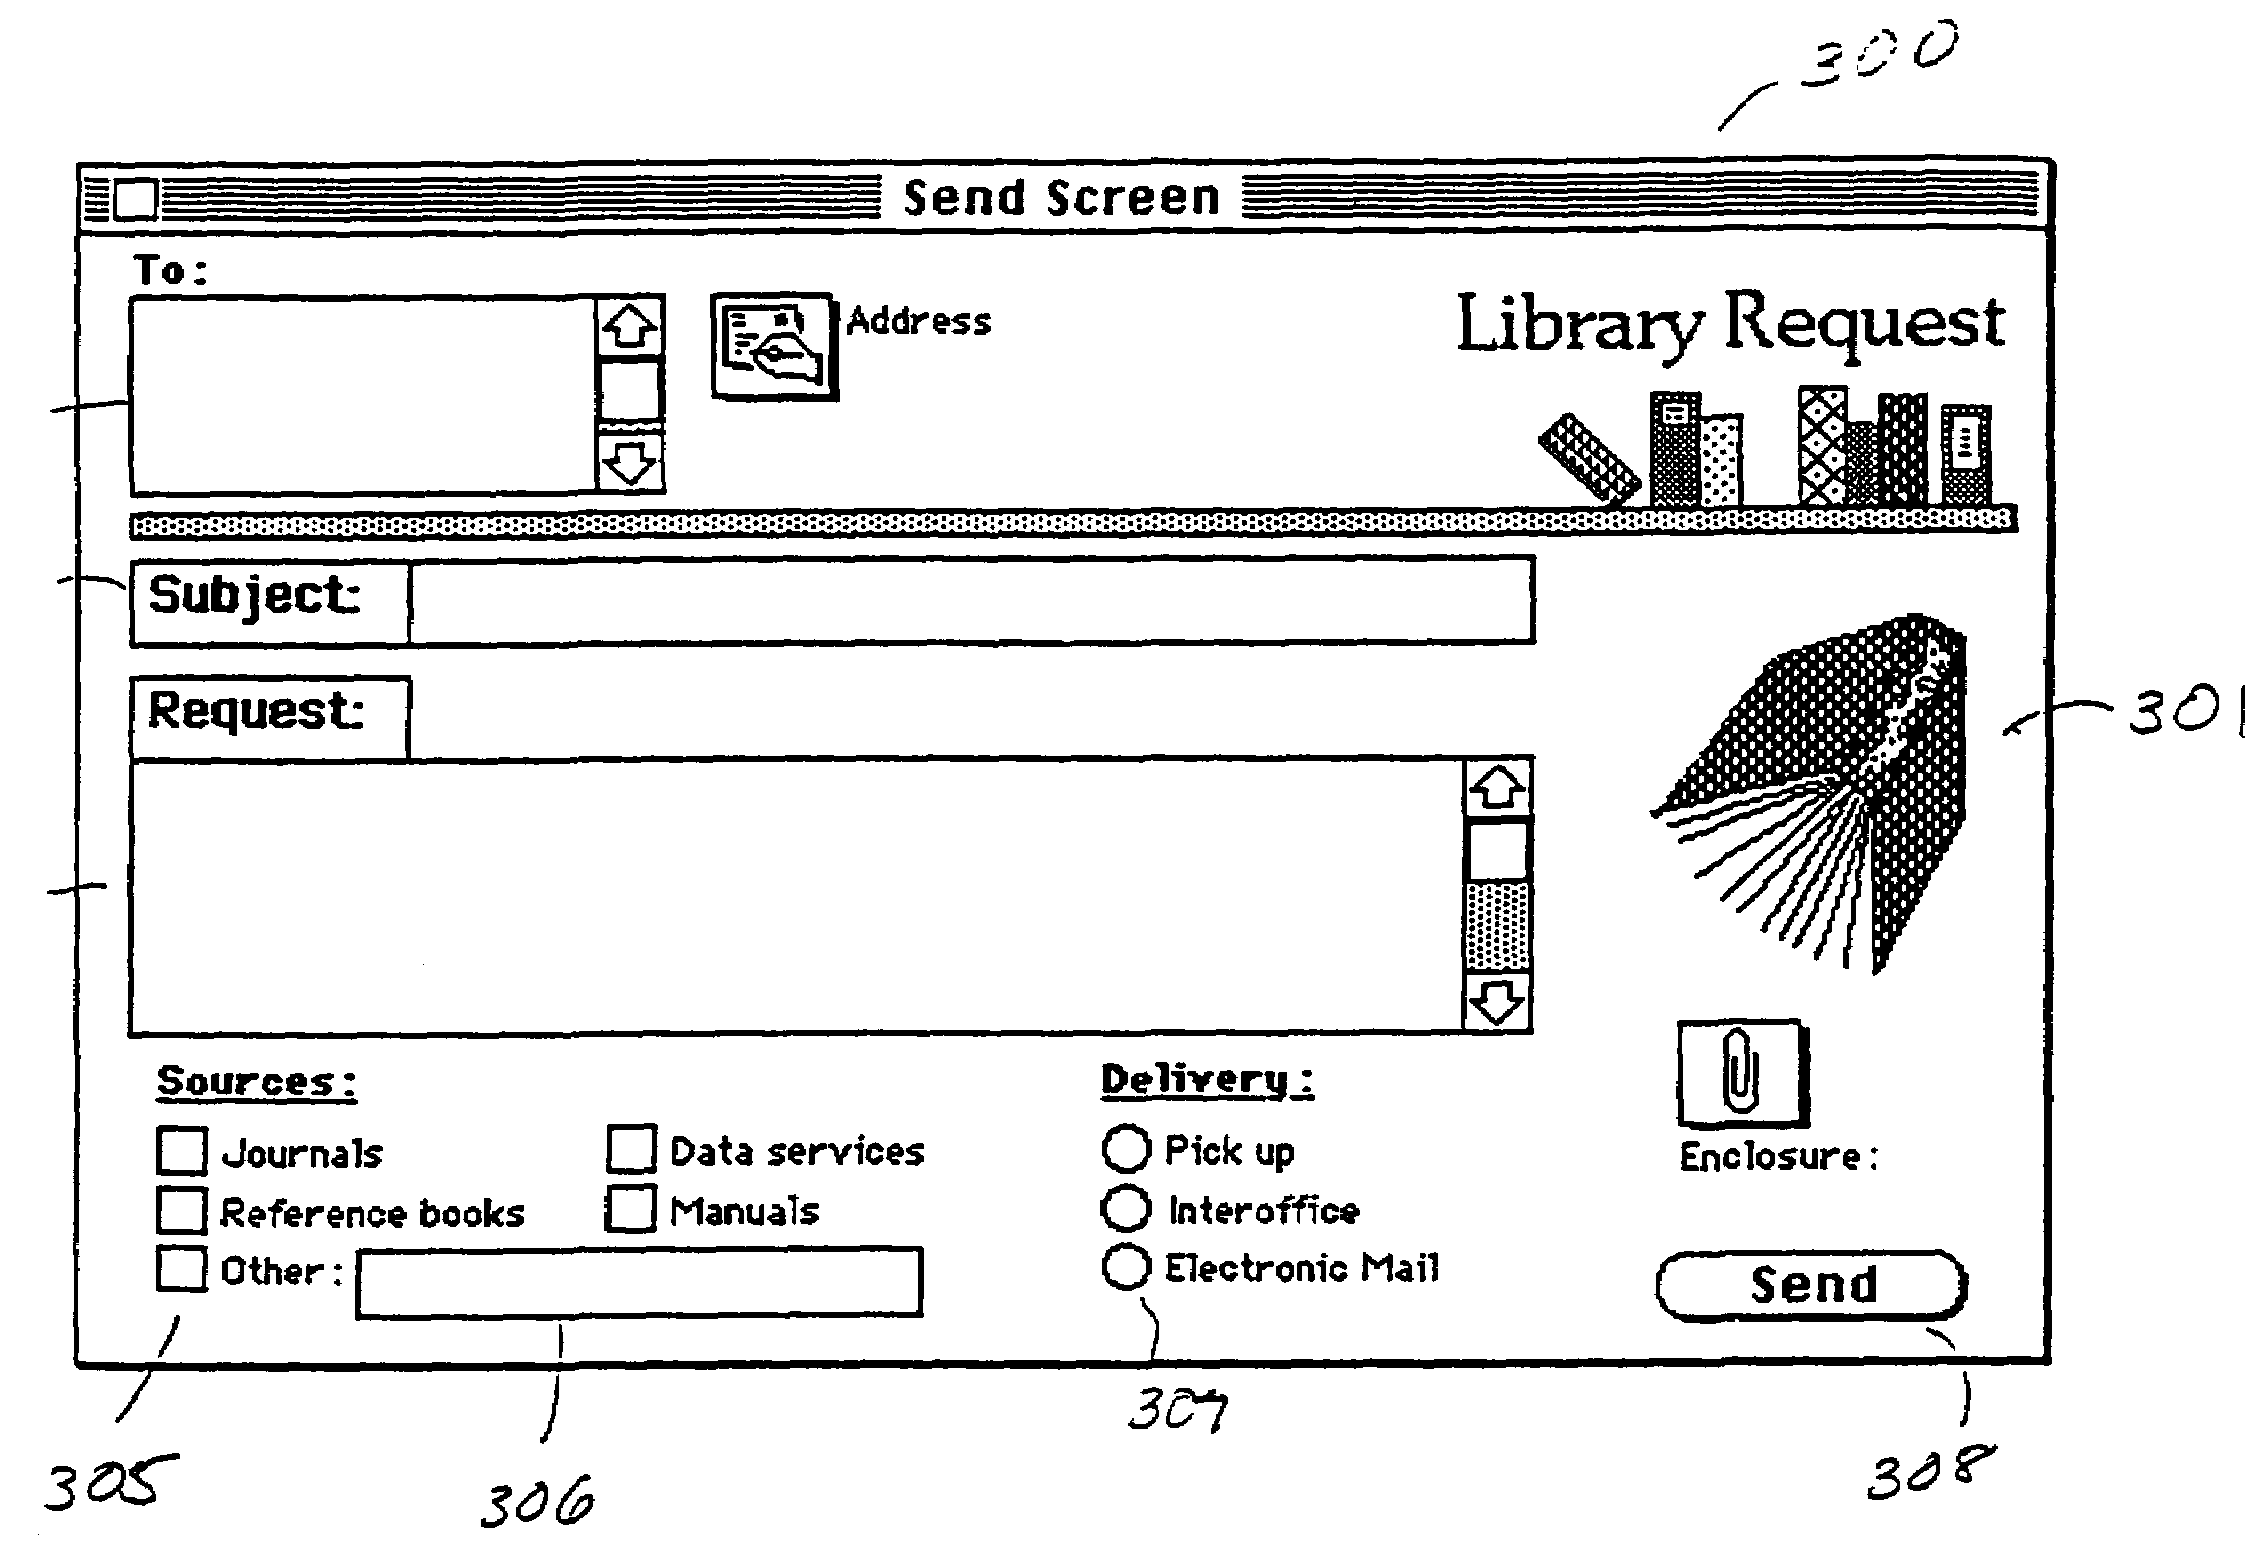
\includegraphics[width=0.7\textwidth]{images/emailform.png}
	\caption{Example Form (Patent \cite{holt_customizing_2006})}
	\label{fig:emailform}
\end{figure}
\end{wrapfigure}

\noindent
forms have a field for address, subject and one for the the actual message to be sent. While an example of what the patent is suggesting can be seen in figure \ref{fig:emailform}, it shows the adding of additional fields allowing for wide variety of form to be created and not force users to use the few forms that are precreated.\\
This increased flexibility in email forms would allow for easier to interpret messages, making responding or providing information via email a lot simpler and quicker.


\subsection{D3: Data Visualisation}
D3 \cite{bostock_d3.js_????} is a javascript library was designed for the creation of interactive visualisations of data and was first developed in 2011. D3 uses precreated Javascript functions to create scalable vector graphics (SVG's) which are embedded into the html of websites."SVG is a language for describing two-dimensional graphics in XML"\cite{ferraiolo_scalable_2000} and can have displays changed  using Cascading Style Sheet (CSS).  \\
Datasets can also be bound to an SVG allowing for visual way to interpret the dataset, and as the dataset changes the SVG will be changed allowing for a dynamic display.  




%%%%%%%%%%%%%%%%%%%%%%%%%%%%%%%%%%%%%%%%%
%										%
%     		 Requirements				%
%										%
%%%%%%%%%%%%%%%%%%%%%%%%%%%%%%%%%%%%%%%%%


\newpage
\section{Requirements}
\newcounter{requirement} \stepcounter{requirement}


\subsection{Functional}
Requirements for the system are each given an idea depending on the type of requirement: FR for functional requirements, NFR for non-functional requirement and SR for system requirements.\\
Along with this, each requirement has a description stating what the requirement is and a priority. The priority value can be low, medium or high, which shows which requirements will be implemented first into the system.


\def\arraystretch{1.5}
\subsubsection{User Requirements}
Functional requirements also include an access column which defines what users should be able to use. Some items are restricted to lecturers as some requirements should only be be usable by lecturers and lab-helpers and not by students.\\
The access levels are: 1-Admin, 2-Lecturers, 3-Lab Helpers and 4-Students




\begin{spacing}{1.2}
\begin{longtable}{|p{0.09\linewidth}|p{0.6\linewidth}|p{0.1\linewidth}|
p{0.1\linewidth}|}
\caption{Functional User Requirements} \label{table:funct-user} \\
\hline


\textbf{ID} & \textbf{Requirement} & \textbf{Access} & \textbf{Priority}\\
\hline \hline


\rid{UR} & Should have to login to view system & 1,2,3,4 & High\\ \hline
\rid{UR} & Should have accounts created for them & 1,2,3,4 & High\\ \hline
\rid{UR} & Should be able to change password & 1,2,3,4 & High\\ \hline
\rid{UR} & Should be able to login using university ID & 1,2,3,4 & Low\\ \hline
\rid{UR} & Should be able to logout & 1,2,3,4 & High \\ \hline

\rid{UR} & Should be able to remove students from courses & 1, 2 & High\\ \hline
\rid{UR} & Should be able to update student accounts & 1,3 & Low \\ \hline

\rid{UR} & Should be able to look up students in lab & 2,3 & High\\ \hline
\rid{UR} & Should be able  to select students from lab list & 2,3 & High\\ \hline
\rid{UR} & Should be able to leave comments about students & 2,3 & High\\ \hline
\rid{UR} & Should be able to search for student by name & 2,3 & Medium\\ \hline
\rid{UR} & Should be able to mark student even if they are not in the system & 2,3 & Medium \\ \hline

\rid{UR} & Should be able to assign students to courses & 1 & Medium\\ \hline
\rid{UR} & Should be able to assign lectures to courses & 1 & Medium \\ \hline

\rid{UR} & Should be able to create marking schemes & 2 & High\\ \hline
\rid{UR} & Should display generated stats & 2 & High\\ \hline
\rid{UR} & Should be able to see submited marks & 2 & High\\ \hline
\rid{UR} & Should be able to generate end of year spread sheets & 2 & Medium\\ \hline
\rid{UR} & Should allow editing of students in class & 2 & Medium\\ \hline
\rid{UR} & Should be able to create peer marking scheme & 2 & Medium\\ \hline
\rid{UR} & Should be able to look at students stats & 2 & Medium\\ \hline
\rid{UR} & Should be able to set what parts of the marking scheme students can see & 2 & Medium\\ \hline
\rid{UR} & Should be able to update marking scheme & 2 & Medium \\ \hline
\rid{UR} & Should be able to able to assign students to set labs & 2 & Low \\ \hline
\rid{UR} & Should be able to set penalties for late marking & 2 & Low \\ \hline

\rid{UR} & Should be able to access Marking Scheme & 3 & High\\ \hline
\rid{UR} & Should be able to enter selected students mark & 3 & High\\ \hline
\rid{UR} & Should be able to submit student mark & 3 & High\\ \hline
\rid{UR} & Should be able to select the lab they are helping in & 3 & High\\ \hline


\rid{UR} & Should be able to see current mark & 4 & High\\ \hline

\end{longtable}
\end{spacing}
\setcounter{requirement}{1}

\newpage
\subsubsection{System Requirements}


All the functional system requirements for the digital marking system are listed in the Table \ref{table:funct-sys}. The systems requirements are functionality that the system should be able to do without users.


\begin{spacing}{1.2}
\begin{longtable}{|p{0.09\linewidth}|p{0.7\linewidth}|p{0.1\linewidth}|}
\caption{Functional System Requirements} \label{table:funct-sys} \\
\hline


\textbf{ID} & \textbf{Requirement} & \textbf{Priority}\\
\hline \hline

\rid{SR} & Should show different displays depending on access level & High\\ \hline
\rid{SR} & Should load students current lab mark scheme & High\\ \hline
\rid{SR} & Should allow marks to updated & High\\ \hline
\rid{SR} & Should apply penalty for late lab completion & High\\ \hline
\rid{SR} & Should create a set of useful stats based on lab & High\\ \hline
\rid{SR} & Should store what class student belong too & High\\ \hline
\rid{SR} & Should have a list of all students in class & High\\ \hline
\rid{SR} & Should list all students that did not attend the lab & Medium\\ \hline
\rid{SR} & Should track how long it takes to mark a student & Medium \\ \hline
\rid{SR} & Should enable results to be importable to vision & Low\\ \hline
\rid{SR} & Should retrieve student Image from university system & Low\\ \hline
\rid{SR} & Should display what students have been marked & Low\\ \hline
\rid{SR} & Should backup database regularly & Low\\ \hline

\rid{SR} & & \\ \hline


\end{longtable}
\end{spacing}
\setcounter{requirement}{1}


\newpage
\subsection{Non-Functional Requirements}

Table \ref{table:non-func} lists all the non-functional requirements for the development of the system. They are ranked in order of priority.


\begin{spacing}{1.2}
\begin{longtable}{|p{0.1\linewidth}|p{0.7\linewidth}|p{0.1\linewidth}|}
\caption{Non-Function Requirements} \label{table:non-func}\\
\hline
\textbf{ID} & \textbf{Requirement} & \textbf{Priority}\\
\hline \hline

\rid{NFR} & Should have all person data encrypted & High\\ \hline
\rid{NFR} & Should update stats as marks are entered & High\\ \hline
\rid{NFR} & Should take less than 2 seconds to generate stats  & High\\ \hline
\rid{NFR} & PHP Should use prepared statements & High\\ \hline
\rid{NFR} & Should be dynamically designed & High\\ \hline
\rid{NFR} & HTML, CSS and Javascript should be validated & High\\ \hline
\rid{NFR} & Should make sure inputs are valid & High\\ \hline
\rid{NFR} & Should prevent SQL Injection & High\\ \hline

\rid{NFR} & Should function on a wide variety of smartphones and tablets & Medium\\ \hline
\rid{NFR} & Should be able to handle a large number of users without any faults & Medium\\ \hline
\rid{NFR} & Should make sure passwords contain alphanumerics and have a minimum and maximum length  & Medium\\ \hline
\rid{NFR} & Should autosave marks as they are entered & Medium\\ \hline
\rid{NFR} & Should record what lab help marked what student & Medium\\ \hline

\rid{NFR} & Should have disability options (Increase text size, colour layout) & Low\\ \hline
\rid{NFR} & Should be readable by screen readers & Low\\ \hline
\rid{NFR} & Should take less than 2 second to load student marking scheme & Low\\ \hline
\rid{NFR} & Test@Test\\ \hline


\end{longtable}
\end{spacing}


\setcounter{requirement}{1}




%%%%%%%%%%%%%%%%%%%%%%%%%%%%%%%%%%%%%%%%%
%										%
%     		Testing & Evaluation		%
%										%
%%%%%%%%%%%%%%%%%%%%%%%%%%%%%%%%%%%%%%%%%
\newpage


\section{Strategy for testing and evaluation}


\subsection{Testing}
During each sprint unit tests will be created and run on modules of code to make sure that they function correctly and to check that the system is ready for the next module to be developed.\\
Each sprint will have set requirements that are to be developed by the end of the sprint. These requirement will each have a test case that will be run at the end of the sprint to make sure that it is successfully implemented.


\subsection{Evaluating}
To evaluate properly how successful I have been at creating a new Lab Marking System I will conduct a usability case study. Lecturers, lab helpers and students will be asked to use the systems and provide feedback, to help evaluate the system and discover what improvements can be made.\\
To evaluate how effective the code is I will create test cases. These will test how efficient the code is at running functions and help find areas for future improvement in the system.





%%%%%%%%%%%%%%%%%%%%%%%%%%%%%%%%%%%%%%%%%
%										%
%     		Project Plan				%
%										%
%%%%%%%%%%%%%%%%%%%%%%%%%%%%%%%%%%%%%%%%%
\newpage
\section{Project Plan and Risk Analysis}


\subsection{Project Plan}


The Gantt chart for this dissertation can be seen in figure(\ref{fig:ganttchart}). It is broken down into 5 stages: Design, Development, Evaluation, Dissertation and Poster. Each of these stages have multiple tasks that are expected to be completed during the course of the stage. A summary of each stage and their key tasks are stated below. \\
\textbf{Design Stage} Starts at the end of semester 1 to allow myself time to complete other course work. In this stage I will create mock-ups for the user interface, a database schema and define what will be occurring in each of my sprints in the next stage.\\
\textbf{Development Stage:} Starts once the holidays are over. It consists of three two week sprints with  a week's break in between to allow for evaluation, write ups and other coursework. When the three sprint finishes I will go straight into the evaluation stage.\\
\textbf{Evaluation Stage: } During the final two weeks before the draft handin, I will conduct a usability case study and write up the remainder of my dissertation for the draft handin.\\
\textbf{Final Deliverable Stage:} This stage  for me is the time to focus on feedback from the draft hand-in and make sure my Dissertation is of a high enough standard.\\
\textbf{Poster Stage:} This stage will be entirely dedicated to the design and creation of my dissertation poster.


\begin{figure}[!htbp]

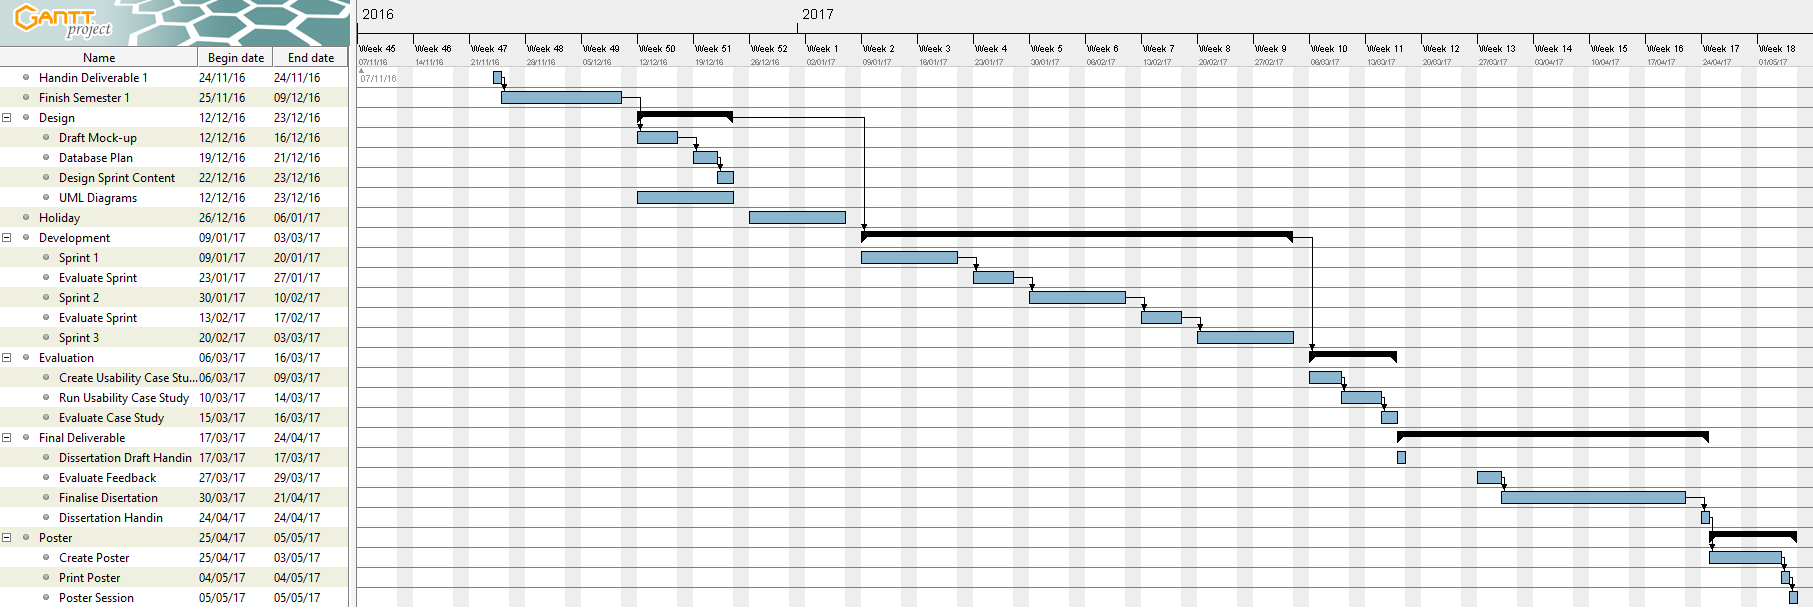
\includegraphics[width=\textwidth]{images/ganttchart.png}
\caption{Project Gantt Chart}
\label{fig:ganttchart}

\end{figure}




%%%%%%%%%%%%%%%%%%%%%%%%%%%%%%%%%%%%%%%%%
%										%
%     		Risk Analysis				%
%										%
%%%%%%%%%%%%%%%%%%%%%%%%%%%%%%%%%%%%%%%%%

\subsection{Risk Analysis}

The risks relating to this dissertation are shown in table(\ref{table:risks}), each risk has an associated Likelihood, Impact and a Mitigation Strategy. Likelihood and Impact values can be low, medium or high. The table is sorted by likelihood and then by the impact

\begin{spacing}{1.2}
\begin{longtable}{|p{0.05\textwidth}|p{0.25\textwidth}|p{0.15\textwidth}|p{0.1\textwidth}|p{0.33\textwidth}|}
\caption{Risk Analysis} \label{table:risks} \\
\hline

\textbf{ID} & \textbf{Risk} & \textbf{Likelihood} & \textbf{Impact } & \textbf{Mitigation Strategy}\\
\hline

\rid{R} & Browsers compatibility & High & High & Constantly test browser compatibility after each sprint\\ \hline

\rid{R} & Other university coursework deadlines & High & Medium & Make sure to allocate adequate amount of time to other courses.\\ \hline



\rid{R} & Lecturers can’t create custom marking schemes & Medium & High & Create selectable forms that lecturers can edit.\\ \hline

\rid{R} & Requirements changed & Medium & Medium & Evaluate requirements before starting development phase and evaluate requirements regularly during project to notice any required changes before it causes a major issue \\ \hline

\rid{R} & System speed is slow & Medium & Medium & Make sure system is well factored and follow coding standards \\ \hline

\rid{R} & Users cannot understand the system & Medium & Medium & Usability Study is being run at the end of the project to evaluation future improvements\\ \hline

\rid{R} & Used libary get updated and causes error & Medium & Medium & Read update information before upgrading to understand where errors might occur\\ \hline

\rid{R} & Admins can’t assign courses & Medium & Medium & Assign courses as part of test data and make note as a future improvement to the system  \\ \hline

\rid{R} & Superviser unable to make meeting & Medium & Low & Contact supervisor and arrange another meeting time \\ \hline

\rid{R} & Cannot get D3 to work & Medium & Low & Just display stats as plain text\\ \hline



\rid{R} & Personal Injury & Low & High & Development would have to be delayed and discussions made with supervisor about how to continue\\ \hline

\rid{R} & Loss of data & Low & High & Back-ups will be stored throughout the project\\
\hline

\rid{R} & Family Issue & Low & High  & Inform MACS and discuss what options are available depending on the situation \\ \hline

\rid{R} & Users can't login & Low & High & Major testing will be done of the login functionality including multiple unit tests\\ \hline

\rid{R} & Users can't log out & Low & Medium & Login will be using sessions which will timeout after a set time so if the user cannot log out then the system do it for them\\ \hline

\rid{R} & Server hosting the project crashes & Low & Medium & Contact the host and enquire about what has happened\\ \hline

\rid{R} & Superviser Leaves & Low & Medium & Inform alisdair and request a new supervisor\\ \hline

\rid{R} & Software Licenses Expire & Low & Low & Check licenses for all software i will be using during the project to make sure they are valid for length of project\\ \hline

\rid{R} & Issues with transport to university  & Low & Low & Use SSH to access any required information at the university  \\ \hline

\end{longtable}
\end{spacing}






%%%%%%%%%%%%%%%%%%%%%%%%%%%%%%%%%%%%%%%%%
%										%
%     			 P.L.E.S				%
%										%
%%%%%%%%%%%%%%%%%%%%%%%%%%%%%%%%%%%%%%%%%
\newpage


\section{P.L.E.S Issues}


\subsection{Professional Issues}
The professional part of this project will be done by following coding standards for the languages that I decide to use.\\
As this project will be a web application I will ensure that both the html and css are validated.\\
The system will be made open source to allow other people to look at and improve the system once I have completed it.\\
The project will be provided with a  user and developer documentation allow for easy development and implementation of the system.


\subsection{Legal Issues}
There are multiple legal issues relating to this project. The most important one is the Data Protection Act. Since the systems will be designed to store data about students I will have to make sure that all data is encrypted and securely stored.\\
I will make sure that I follow the terms and services for any software or libraries I used as part of the project, as to make sure I am not breaking any laws.


\subsection{Ethical Issues}
A major ethical requirement of this project is to do with the storage of students personal information on a digital system; to deal with this issue I should consult the data protection act. \\
Another issue that is raised by this project is making sure that students are not deceived and that the marks they see are actually the ones they have received.\\
The last ethical issue relating to this project is making sure that students are online able to see their own mark and cannot see another student's mark. It should also be made such that final grades are only visible to the lecture and student keeping it confidential from lab helpers.


\subsection{Social Issues}
A few social issues are raised by this project. Such as if students can see the mark they have received straight away, will lab helpers feel pressurised into giving higher grades.\\
Will this system result in a reduction of lab helpers being required to mark labs? If the system speeds up the time to mark students’ work, less lab helpers may be required to run labs, resulting in people looking for work.






%%%%%%%%%%%%%%%%%%%%%%%%%%%%%%%%%%%%%%%%%
%										%
%     		Bibliography				%
%										%
%%%%%%%%%%%%%%%%%%%%%%%%%%%%%%%%%%%%%%%%%

\newpage
\printbibliography[heading=bibintoc]


\end{document}